\documentclass{article}
\usepackage[utf8]{inputenc}
\usepackage[T5]{fontenc}
\usepackage[fontsize=13pt]{scrextend}
\usepackage[paperheight=29.7cm,paperwidth=21cm,right=2cm,left=3cm,top=2cm,bottom=2.5cm]{geometry}
\usepackage{mathptmx}
\usepackage{amsfonts}
\usepackage{amssymb}
\usepackage{mathtools}
\usepackage{graphicx}
\usepackage{float}
\usepackage{tikz}
\usetikzlibrary{calc}
\usepackage{indentfirst} %thư viện thụt đầu dòng
\renewcommand{\baselinestretch}{1.2} %dãn dòng 1.2cm
\setlength{\parskip}{6pt} %dãn dòng giữa các đoạn văn
\setlength{\parindent}{1cm} %xét khoảng cách thụt đầu dòng
\usepackage{titlesec} %thư viện setup các kiểu chữ
\setcounter{secnumdepth}{4} %4 heading
\titlespacing*{\section}{0pt}{0pt}{30pt} %setup heading1
\titleformat*{\section}{\fontsize{16pt}{0pt} \selectfont \bfseries \centering}

\titlespacing*{\subsection}{0pt}{10pt}{0pt} %setup heading2
\titleformat*{\subsection}{\fontsize{14pt}{0pt}\selectfont \bfseries}

\titlespacing*{\subsubsection}{0pt}{10pt}{0pt} %setup heading3
\titleformat*{\subsubsection}{\fontsize{13pt}{0pt}\selectfont \bfseries \itshape}

\titlespacing*{\paragraph}{0pt}{10pt}{0pt} %setup heading4
\titleformat*{\paragraph}{\fontsize{13pt}{0pt}\selectfont \itshape}
\renewcommand{\theequation}{\thesection.\arabic{equation}} 
\renewcommand{\figurename}{\fontsize{12pt}{0pt}\selectfont \bfseries Hình} %thay đổi Figure --> Hình
\renewcommand{\theequation}{\thesection.\arabic{equation}} % Thay đổi đánh số phương trình mặc định
\renewcommand{\thefigure}{\thesection.\arabic{figure}} %thay đổi đánh số mặc định
\usepackage{caption}
\captionsetup[figure]{labelsep=space}

\renewcommand{\tablename}{\fontsize{12pt}{0pt}\selectfont \bfseries Bảng}
\renewcommand{\thetable}{\thesection.\arabic{table}}
\captionsetup[table]{labelsep=space}

\usepackage[most]{tcolorbox}
\usepackage{minted}
\usepackage{tabularx}
\newcolumntype{s}{>{\hsize=.5\hsize}X} %cột S = 0.4 lần cột X
\newcolumntype{a}{>{\hsize=1\hsize}X}
\newcolumntype{H}{>{\hsize=1\hsize}X} %cột S = 0.4 lần cột X
\newcolumntype{K}{>{\hsize=1\hsize}X}
\newcolumntype{M}{>{\hsize=.6\hsize}X}%cột S = 0.4 lần cột X
\newcolumntype{N}{>{\hsize=1.4\hsize}X}

\renewcommand{\theequation}{\thesection.\arabic{equation}}%thay đổi đánh số pt mặc định
\newtheorem{theorem}{Định lý}[section] %đánh số định lý
\newtheorem{defn}[theorem]{Định nghĩa} %đánh số định nghĩa
\newtheorem{corollary}[theorem]{Hệ quả}
\newtheorem{lemma}[theorem]{bổ đề}

\usepackage{amsmath} % thư viện tạo ma trận toán học
\usepackage{lipsum} % thư viện tạo chữ linh tinh làm ví dụ

\renewcommand{\contentsname}{MỤC LỤC}
\renewcommand{\listfigurename}{DANH MỤC HÌNH VẼ}
\renewcommand{\listtablename}{DANH MỤC BẢNG BIỂU}
\renewcommand{\refname}{TÀI LIỆU THAM KHẢO}

\usepackage[unicode]{hyperref}

\usepackage{hyperref}

\begin{document}
\begin{titlepage}
\begin{tikzpicture}[overlay,remember picture]
\draw [line width=3pt]
    ($ (current page.north west) + (3.0cm,-2cm) $)
    rectangle
    ($ (current page.south east) + (-2.0cm,2.5cm) $);
\draw [line width=0.5pt]
    ($ (current page.north west) + (3.1cm,-2.1cm) $)
    rectangle
    ($ (current page.south east) + (-2.1cm,2.6cm) $);
\end{tikzpicture}
\begin{center}
\vspace{-20pt}    TRƯỜNG ĐẠI HỌC BÁCH KHOA HÀ NỘI \\
\textbf{\fontsize{16pt}{0pt}\selectfont VIỆN ĐIỆN TỬ - VIỄN THÔNG}
\vspace{0.5cm}
\begin{figure}[H]
    \centering
    
\includegraphics[height=2.26cm,width=1.53cm]{images/Logo_Hust.png}
\end{figure}
\vspace{2cm}
\fontsize{16pt}{0pt}\selectfont BÁO CÁO BÀI TẬP LỚN \\
\vspace{12pt}
\textbf{\fontsize{32pt}{0pt}\selectfont THÔNG TIN DI ĐỘNG\\}
\vspace{5pt}
%\textbf{\fontsize{32pt}{0pt}\selectfont AND PRESENTATION}
\vspace{40pt}

\end{center}
\hspace{6pt} \textbf{\fontsize{14pt}{0pt}\selectfont Đề tài:}
\begin{center}
    \textbf{\fontsize{20pt}{0pt}\hspace{5pt}\selectfont THỰC HIỆN ĐIỀU CHẾ, MÃ HÓA, GIẢI MÃ HÓA LDPC CHO MẠNG DI ĐỘNG 4G \\}
    \vspace{5pt}
%    \textbf{\fontsize{20pt}{0pt}\selectfont ON SYSTEM-ON-A-CHIP DESIGNS\\}
\vspace{2.0cm}
\begin{table}[H]
    \centering
\begin{tabular}{l l}
    \fontsize{14pt}{0pt}\selectfont Sinh viên thực hiện: & \fontsize{14pt}{0pt}\selectfont VŨ THÀNH TRUNG- 20186319 \vspace{6pt} \\
    &  \fontsize{14pt}{0pt}\selectfont NGUYỄN VIỆT HOÀNG - 20186315 \vspace{6pt} \\
    &  \fontsize{14pt}{0pt}\selectfont VŨ HIẾU TRUNG - 20182839 \vspace{6pt} \\
    \fontsize{14pt}{0pt}\selectfont Nhóm: & \fontsize{14pt}{0pt}\selectfont 1 \\
    \fontsize{14pt}{0pt}\selectfont Giảng viên hướng dẫn: &\fontsize{14pt}{0pt}\selectfont PGS.TS. NGUYỄN VĂN ĐỨC \\
\end{tabular}
\end{table}
\vspace{2.5cm}
 \fontsize{14pt}{0pt}\selectfont Hà Nội, 1-2022
\end{center}
\end{titlepage}

\section*{LỜI NÓI ĐẦU}
\thispagestyle{empty}
Hệ thống thông tin di động thế hệ thứ 4 (4G - 4th Generation) cần đạt được cả 3 tiêu chí chính là băng thông rộng, độ tin cậy cao và độ trễ thấp. Mã kiểm tra chẵn lẻ mật độ thấp (LDPC - Low Density Parity Check) đã được chấp nhận cho hệ thống thông tin di động 4G vì mã LDPC gần đạt được dung lượng Shannon. Trong báo cáo này, chúng em mô phỏng bộ mã LDPC bằng Matlab trên kênh truyền nhiễu trắng(AWGN) với phương pháp điều chế BPSK để chứng minh tính hiệu quả của bộ mã này trong cho hệ thống thông tin di động 4G.

\cleardoublepage
\addtocontents{toc}{\protect\thispagestyle{empty}}
\tableofcontents % tạo mục lục tự động
\thispagestyle{empty}
\cleardoublepage

\pagenumbering{roman}%đánh số thứ tụ la mã

\section*{DANH MỤC KÍ HIỆU VÀ CHỮ VIẾT TẮT}
\phantomsection \addcontentsline{toc}{section}{\numberline {}DANH MỤC KÍ HIỆU VÀ CHỮ VIẾT TẮT}
\begin{table}[H]
    \centering
    \begin{tabularx}{0.8\textwidth}
    {
    |>{\centering\arraybackslash}M
    |>{\centering\arraybackslash}N|
    }
    \hline
      \bfseries Kí hiệu  &  \bfseries Giải nghĩa \\ \hline
        LDPC   & Low - density Parity Check   \\ \hline
        AWGN & White Noise Gauss \\ \hline
        DVB  & Digital Video Broadcasting   \\ \hline
        NR    &  New Radio\\ \hline
        BG   &  Base Graph \\ \hline
        SPC   &  Single Parity Check \\ \hline
        ML   &  Maximum Likelihood \\ \hline
        BPSK & Binary Phase Shift Keying  \\ \hline
    \end{tabularx}
\end{table}
\cleardoublepage

{\let\oldnumberline\numberline
\renewcommand{\numberline}{\figurename~\oldnumberline}
\listoffigures}%tạo danh mục hình vẽ
\phantomsection \addcontentsline{toc}{section}{\numberline{}DANH MỤC HÌNH VẼ}
\cleardoublepage
{\let\oldnumberline\numberline
\renewcommand{\numberline}{\tablename~\oldnumberline}
\listoftables} %tạo danh mục hình vẽ
\phantomsection \addcontentsline{toc}{section}{\numberline{}DANH MỤC BẢNG BIỂU}
\cleardoublepage

\pagenumbering{arabic} %đánh số thứ tự 1,2 ,3,4.....
\section*{CHƯƠNG 1. CƠ SỞ LÝ THUYẾT}
\addcontentsline{toc}{section}{\numberline{}CHƯƠNG 1. CƠ SỞ LÝ THUYẾT}
\setcounter{section}{1}
\setcounter{subsection}{0}
\setcounter{figure}{0}
\setcounter{table}{0}
\subsection{Khái niệm LDPC }

Mã LDPC (Low - density Parity Check) mã kiểm tra chẵn lẻ mật độ thấ , hay còn gọi là mã Gallager, được đề xuất bởi Gallager vào năm 1962. Với ưu thế chính là khả năng sửa lỗi đạt gần giới hạn Shannon trên kênh đối xứng nhị phân (BSC) cũng như trên kênh White Noise Gauss  (AWGN), mã LDPC đã thu hút được nhiều sự quan từ cộng đồng nghiên cứu lẫn giới công nghệ và được ứng dụng trong các công nghệ hiện nay, điển hình như là: Wireless, DVB (Digital Video Broadcasting), 5G NR (New Radio)…  Về cơ bản, mã LDPC là một loại mã khối tuyến tính sử dụng ma trận kiểm tra chẵn lẻ các ma trận thưa (Sparse Parity-check Matrix), tức là hầu hết các phần tử là 0, chỉ một số ít là 1. Theo định nghĩa của Gallager, ma trận kiểm tra chẵn lẻ của mã LDPC có đặc điểm là mỗi hàng chứa đúng i phần tử 1 và mỗi cột chứa đúng j phần tử 1. Bằng việc sử dụng phương pháp truyền tin tưởng lặp (Iterative Belief  Propagation) LDPC có thể được giải mã thời gian tuyến tính theo chiều dài khối của chúng.

Mã LDPC đang được sử dụng ngày càng nhiều trong các ứng dụng yêu cầu truyền thông tin đáng tin cậy và hiệu quả cao qua các liên kết giới hạn băng thông hoặc giới hạn kênh trả về khi có sự xuất hiện của nhiễu.

\subsection{Cấu trúc của mã LDPC}
Về cơ bản, một mã LDPC đều là 1 loại mã khối tuyến tính mà mã trận kiểm tra chẵn lẻ H(mxn) có trọng số cột g và trọng số hàng r sao cho r = g(n/m) và g<<m. Nếu H có mật độ thấp và trọng số cột, hàng không phải là hằng số, thì mã đó sẽ là mã LDPC không đều. Ví dụ dưới đây là ma trận 6x12 đều có trọng số cột là 3, trọng số hàng là 6.

\begin{equation*}
\setcounter{MaxMatrixCols}{20}
H = 
\begin{bmatrix}
1 & 1 & 1 & 0 & 0 & 1 & 1 & 0 & 0 & 0 & 1 & 0 \\
1 & 1 & 1 & 1 & 1 & 0 & 0 & 0 & 0 & 0 & 0 & 1 \\
0 & 0 & 0 & 0 & 0 & 1 & 1 & 1 & 0 & 1 & 1 & 1 \\
1 & 0 & 0 & 1 & 0 & 0 & 0 & 1 & 1 & 1 & 0 & 1 \\
0 & 1 & 0 & 1 & 1 & 0 & 1 & 1 & 1 & 0 & 0 & 0 \\
0 & 0 & 1 & 0 & 1 & 1 & 0 & 0 & 1 & 1 & 1 & 0 \\
\end{bmatrix}
\end{equation*}

Base graph (base matrix): Là ma trận cơ sở mà từng phần tử trong ma trận có thể được mở rộng ra dựa vào hệ số mở rộng Z. Nói cách khác, ma trận cơ sở sẽ chứa các giá trị dịch chuyển $P_{i_j}$, -1 $\le$ $P_{i_j}$ $\le$ Z-1, với mỗi giá trị dịch chuyển $P_{i_j}$ sẽ có thể chuyển đổi thành ma trận đơn vị I có kích thước $Z$x$Z$ dịch chuyển sang phải $P_{i_j}$ lần  đối với phần tử $(i,j)^{th}$ $\ne$ 0 trong ma trận cơ sở. Ma trận hoán vị tuần hoàn nhị phân này sẽ được ký hiệu là $ Q(P_{i_j})$.

\begin{equation*}
\setcounter{MaxMatrixCols}{20}
Q(1) = 
\begin{bmatrix}
0 & 1 & 0 & \cdots & 0 \\
0 & 0 & 1 & \cdots & 0 \\
\vdots  & \vdots  & \ddots & \vdots  \\
0 & 0 & 0 & \cdots & 1 \\ 
1 & 0 & 0 & \cdots & 0 \\ 
\end{bmatrix}
\end{equation*}
Ví dụ trên là ma trận Q(1) dịch chuyển sang phải 1 lần. Do đó, Q(-1) để hiển thị ma trận rỗng, tất cả các phần tử bằng 0.

Từ đây, ta có thể xác định được ma trận kiểm tra chẵn lẻ dựa trên ma trận cơ sở và hệ số dịch chuyển $P_{i_j}$ trong ma trận cơ sở. Các phần tử trong ma trận cơ sở (có giá trị từ -1 ->  Z – 1) sẽ được thay thế bằng các ma trận hoán vị tuần hoàn nhị phân tương ứng theo phương pháp mở rộng bên trên.
\begin{equation*}
\setcounter{MaxMatrixCols}{20}
H = 
\begin{bmatrix}
$$Q(P_{1,1})$$ & $$Q(P_{1,2})$$ & \cdots & $$Q(P_{1,n_b})$$ \\
$$Q(P_{2,1})$$ & $$Q(P_{2,2})$$ & \cdots & $$Q(P_{2,n_b})$$\\
\vdots  & \vdots  & \ddots & \vdots  \\
$$Q(P_{m_b,1})$$ & $$Q(P_{m_b, 2})$$ & \cdots & $$Q(P_{m_b,n_b})$$ \\ 
\end{bmatrix}
\end{equation*}
H là ma trận kiểm tra chẵn lẻ cho ma trận có kích thước $m_b$x$n_b$

Ta có ma trận cơ sở của ma trận H như sau:
\begin{equation*}
\setcounter{MaxMatrixCols}{20}
E(H) = 
\begin{bmatrix}
$$P_{1,1}$$ & $$P_{1,2}$$ & \cdots & $$P_{1,n_b}$$ \\
$$P_{2,1}$$ & $$P_{2,2}$$ & \cdots & $$P_{2,n_b}$$ \\
\vdots  & \vdots  & \ddots & \vdots  \\
$$P_{m_b,1}$$ & $$P_{m_b, 2}$$ & \cdots & $$P_{m_b,n_b}$$ \\ 
\end{bmatrix}
\end{equation*}

Cấu trúc khối của ma trận cơ sở sẽ có dạng như hình dưới đây
\begin{figure}[H]
    \centering
    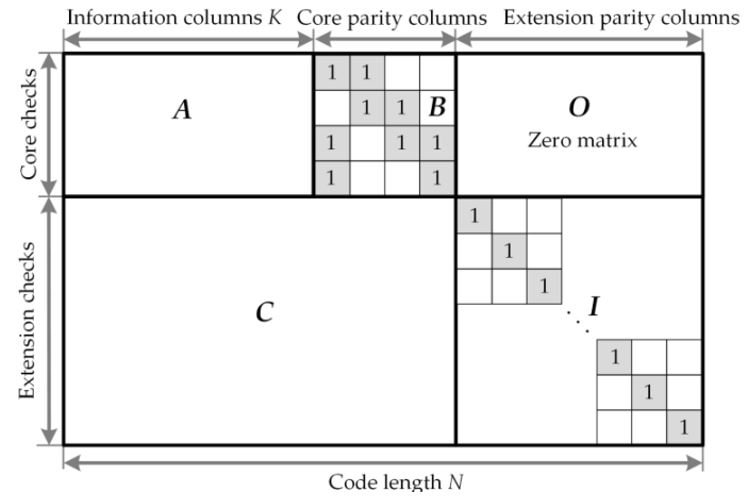
\includegraphics[width=10cm]{images/Matrancoso.JPG}
    \caption[Cấu trúc của ma trận cơ sở]{\bfseries\fontsize{12pt}{0pt} \selectfont Cấu trúc của ma trận cơ sở} %[tên ở list figure]{tên chú thích ảnh}
    \label{hinh11}
\end{figure}
\begin{itemize}
    \item  Các cột trong ma trận cơ sở sẽ được chia làm 3 phần: Cột thông tin, cột chẵn lẻ cốt lõi (hay đường chéo kép) và cột chẵn lẻ mở rộng. Các hàng trong ma trận cơ sở được chia làm 2 phần: Hàng kiểm tra cốt lõi và hàng kiểm tra mở rộng. Như ở hình trên, ma trận cơ sở sẽ gồm các ma trận con A,B,O,C và I. Ma trận con A sẽ tương ứng với các bit có tính hệ thống. Ma trận con B tương ứng với tập hợp bit chẵn lẻ đầu tiên có cấu trúc đường chéo kép. Ma trận con O là ma trận 0. Các ma trận con C và I được dùng để hỗ trợ cho việc nhanh chóng yêu cầu lặp lại tự động, kết hợp gia tăng dự phòng. A và B được coi là hạt nhân, còn O, C và I được coi là phần mở rộng.
    \item 3GPP đưa ra 2 cấu trúc ma trận cơ sở chính cho việc mã hóa kênh là BG1 có ma trận H kích thước 46x68 và BG2 có ma trận H kích thước 42x52.
    \item BG1 có độ dài lớn hơn và tỷ lệ mã hóa R cao hơn. Nếu kích thước khối $\le$ 292 hoặc $\le$ 3824 và R $\le$ 2/3 hoặc R $\le$ 1/4 thì ma trận cơ sở 2, BG2, của mã LDPC được sử dụng; nếu không thì ma trận cơ sở 1, BG1, của mã LDPC được sử dụng.
    \begin{figure}[H]
    \centering
    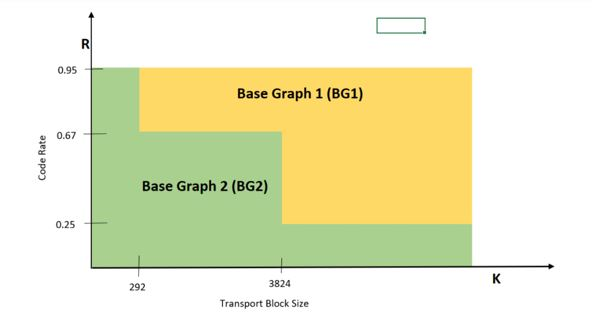
\includegraphics[width=10cm]{images/3gpp.JPG}
    \caption[Cách lựa chọn cấu trúc ma trận cơ sở theo 3GPP]{\bfseries\fontsize{12pt}{0pt} \selectfont Cách lựa chọn cấu trúc ma trận cơ sở theo 3GPP} %[tên ở list figure]{tên chú thích ảnh}
    \label{hinh12}
\end{figure}
    \item Đối với các ma trận BG1 và BG2 thì số lượng thiết kế hệ số dịch chuyển là 8. Tất cả các kích thước khác được chia thành 8 tập dựa trên tham số a, trong đó a được sử dụng để xác định hệ số mở rộng $Z = a$ × $ 2^j$.
    
  \begin{table}[H]
    \centering
    \caption[Tập các hệ số mở rộng]{\bfseries Tập các hệ số mở rộng}
    \label{bang11}
    \begin{tabularx}{9.9cm} {|c|c|}
  \hline
  \textbf{Ma trận lũy thừa} & \textbf{Tập kích thước nâng}  \\ \hline
   Tập 1 & $Z = 2 x 2^j, j=0,1,2,3,4,5,6,7$  \\ \hline
   Tập 2 & $Z = 3 x 2^j, j=0,1,2,3,4,5,6,7$ \\ \hline
   Tập 3 & \hspace{-0.4cm} $Z = 5 x 2^j, j=0,1,2,3,4,5,6$  \\ \hline
   Tập 4 & \hspace{-0.7cm} $Z = 7 x 2^j, j=0,1,2,3,4,5$\\ \hline
   Tập 5 & \hspace{-0.8cm} $Z = 9 x 2^j, j=0,1,2,3,4,5$\\ \hline
   Tập 6 & \hspace{-0.6cm} $Z = 11 x 2^j, j=0,1,2,3,4,5$ \\ \hline
   Tập 7 & \hspace{-0.9cm} $Z = 13 x 2^j, j=0,1,2,3,4$  \\ \hline
   Tập 8 & \hspace{-0.9cm} $Z = 15 x 2^j, j=0,1,2,3,4$ \\\hline
     \end{tabularx}
  \end{table}
    
    \item Giá trị hệ số dịch chuyển $P_{ij}$  có thể được tính bằng cách sử dụng hàm  $P_{ij}$ = $f$($V_{ij}$, $Z$), trong đó $V_{ij}$ là hệ số dịch chuyển của phần tử $(i, j)$. Hàm $f$   được định nghĩa như sau:
    
    \begin{equation}\label{pt11}
    P_{i,j} = f(V_{i,j}, Z) =
    \Bigg \{ \begin{matrix}
        -1, \hspace{0.6cm}  $$V_{i,j}$$, $Z$ = -1 \\
        mod($$V_{i,j}$$, $Z$),    \hspace{0.6cm}  khac
    \end{matrix}
    \end{equation}
    Trong đó, mod là toán tử của phép module.
    \end{itemize}
\subsection{Cấu trúc của mã LDPC}
    \begin{itemize}
      \item Thay vì sử dụng ma trận sinh G như với SPC (Single Parity Check), mã LDPC có thể được mã hóa sử  dụng trực tiếp bằng ma trận chẵn lẻ H.

      \item Cho từ mã $C = [s, p_a, p_c]$, trong đó s biểu thị phần hệ thống, được chia thành kb nhóm gồm Z bits vì mô hình cơ sở có $k_b = n_b - m_b$ cột bit thông tin. Hơn nữa, $s=[s1,s2,...,s_{kb}]$ trong đó mỗi phần tử của s là một vector có độ dài Z. Các bản tin nhận được bởi bộ mã hóa được lưu trữ trong các thanh ghi được sắp xếp theo khối $k_b$, ký hiệu là $s_i (i = 1, 2, ..., k_b)$, tương ứng với các khối hệ thống, trong đó mỗi khối bao gồm Z bit. Giả sử rằng phần chẵn lẻ của mỗi thông tin p được chia thành 2 thành phần như sau: g = 4 bit chẵn lẻ đầu tiên ,$p_a=[p_{a1}, p_{a2},...,p_{ag}]$ và phần còn lại gồm $(m_b-g)$ bit kiểm tra $p_c=[p_{c1} ,p_{c2},...,p_{c(mb-g)}]$.
      
      \item  Cụ thể, từ mã mã hóa được biểu diễn như sau:
      \begin{equation}\label{pt12}
         C = [s_1,s_2,...,skb, p_{a1}, p_{a2},...,p_{ag}, p_{c1}, p_{c2},...,p_{c(mb-g)]}
      \end{equation}
      
      \item	Ma trận chẵn lẻ H của LDPC được chia thành 6 ma trận con:
      \begin{equation}\label{pt13}
         H = 
         \begin{bmatrix}
          A & B & 0 \\
          C_1 & C_2 & I \\ 
        \end{bmatrix}
      \end{equation}
      Trong đó: A là ma trận có kích thước g×kb, B là ma trận có kích thước $g×g$, C1 là ma trận có kích thước $$(m_b-g)×k_b$$ và C2 là ma trận có kích thước $$(m_b-g)×g$$. Ngoài ra, I là một ma trận đơn vị có kích thước là $$(m_b-g)×( m_b-g)$$. Việc mã hóa các mã LDPC được thực hiện bằng cách sử dụng phương trình sau: 
        \begin{equation}\label{pt14}
         HC^T= 0^T
        \end{equation}
     \item  Phương trình trên được biểu thị như sau:
      \begin{equation}\label{pt15}
          \begin{bmatrix}
            A & B & 0 \\
            C_1 & C_2 & I \\ 
          \end{bmatrix}
        \begin{bmatrix}
            s \\
           p_a \\
           p_c
          \end{bmatrix}
           = 0^T 
      \end{equation}
      \item  Từ phương trình trên ta thu được hai phương trình sau:
        \begin{equation}\label{pt16}
         As^T+Bp_a^T+0p_a^T = 0^T
      \end{equation}
      \begin{equation}\label{pt17}
         C_1s^T + C_2p_a^T + Ip_a^T = 0^T		
      \end{equation}
      
      \item 	Bước đầu tiên trong việc triển khai bộ mã hóa là xác định phần $p_a$. Trước tiên, phương trình (1.6) được viết lại ở dạng khối như sau:
        \begin{equation}\label{pt18}
          \begin{bmatrix}
            a_{1,1} & a_{1,2} & \cdots & a_{1,k_b} \\
            a_{2,1} & a_{2,2} & \cdots & a_{2,k_b} \\
            a_{3,1} & a_{3,2} & \cdots & a_{3,k_b} \\
            a_{4,1} & a_{4,2} & \cdots & a_{4,k_b} 
          \end{bmatrix}
          \begin{bmatrix}
             s_1 \\
             s_2 \\
             \cdots \\
             s_{kb} 
          \end{bmatrix}
           +  
           \begin{bmatrix}
            1 & 0 & -1 & -1 \\
            0 & 0 & 0 & -1 \\
            -1 & -1 & 0 & 0 \\
            1 & -1 & -1 & 0 \\
          \end{bmatrix}
          \begin{bmatrix}
           {p_a}_1 \\
           {p_a}_2\\
           {p_a}_3\\
           {p_a}_4 
          \end{bmatrix}
           = 0
      \end{equation}
      \item  Sau đó, mở rộng phương trình (1.8) thành tập phương trình sau:
      \begin{equation}\label{pt19}
         \displaystyle \sum_{j=1}^{k_b} a_{1,j}S_j + {p_a}_1 ^{(1)} + {p_a}_2 = 0^T
      \end{equation}
      \begin{equation}\label{pt120}
        \hspace{1cm}\displaystyle \sum_{j=1}^{k_b} a_{2,j}S_j + {p_a}_1 + {p_a}_2 + {p_a}_3= 0^T	
      \end{equation}
      \begin{equation}\label{pt121}
         \displaystyle \sum_{j=1}^{k_b} a_{3,j}S_j + {p_a}_3 + {p_a}_4 = 0^T	
      \end{equation}
      \begin{equation}\label{pt122}
         \hspace{0.3cm}\displaystyle \sum_{j=1}^{k_b} a_{4,j}S_j + {p_a}_1 ^{(1)} + {p_a}_4 = 0^T	
      \end{equation}
      \item Trong đó ${p_a}_1 ^{(1)}$ biểu thị phiên bản dịch chuyển sang phải 1 của ${p_a}_1$.
      \item Bằng cách cộng tất cả các phương trình trên ta được:
        \begin{equation}\label{pt123}
            {p_a}_1 = \sum_{i=1}^{4} \sum_{j=1}^{k_b} a_{(i,j)} S_j
        \end{equation}
      \item Ta có thể viết lại như sau:
       \begin{equation}\label{124}
            \hspace{2.8cm}\lambda_i = \sum_{j=1}^{k_b} a_{i,j}S_j  \hspace{10pt} với \hspace{15pt} i=1,2,3,4
       \end{equation}
       \begin{equation}\label{125}
           \hspace{-0.9cm}{p_a}_1 = \sum_{i=1}^{4} \lambda_i
       \end{equation}
       \begin{equation}\label{126}
           {p_a}_2 = \lambda_1 + {p_a}_1 ^{(1)}
       \end{equation}
       \begin{equation}\label{127}
          \hspace{-0.4cm} {p_a}_3 = \lambda_3 + {p_a}_4
       \end{equation}
       \begin{equation}\label{128}
           {p_a}_4 = \lambda_4 + {p_a}_1 ^{(1)}
       \end{equation}
       \item  Từ phương trình (1.14), mỗi giá trị của $lambda_i$ được tính bằng cách cộng dồn tất cả các giá trị của $a_(i,j)S_j$. Trong phép toán modulo, $lambda_i$ được tính bằng cách thực hiện phép toán XOR trên tất cả các phần tử của $a_(i,j)S_j$. Khối thứ nhất của bit chẵn lẻ ${p_a}_1$ được tính bằng cách tích lũy tất cả các giá trị $lambda_i$. Các bit chẵn lẻ còn lại có thể lấy được dựa vào phương trình (1.15)-(1.18). Tất cả các bit chẵn lẻ đầu tiên pa được lưu giữ trong thanh ghi dịch.
       \item  Tiếp theo, ta xác định $p_c$ dựa trên phương trình (7), trong đó ma trận $C_1$ và $C_2$ được cho bởi 
       \begin{equation}\label{129}
           C_1 = 
          \begin{bmatrix}
            C_{1,1} & C_{1,2} & \cdots & C_{1,k_b} \\
            C_{2,1} & C_{2,2} & \cdots & C_{2,k_b} \\
            \vdots  & \vdots  & \ddots & \vdots  \\
            C_{mb-g,1} & C_{mb-g,2} & \cdots & C_{mb-g,k_b}\\
          \end{bmatrix}
       \end{equation}
       \begin{equation}\label{130}
           C_2 = 
          \begin{bmatrix}
            C_{1,{k_b}+1} & C_{1,{k_b}+2} & \cdots & C_{1,{k_b}+g} \\
            C_{2,{k_b}+1} & C_{2,{k_b}+2} & \cdots & C_{2,{k_b}+g} \\
            \vdots  & \vdots  & \ddots & \vdots  \\
            C_{mb-g,{k_b}+1} & C_{mb-g,{k_b}+2} & \cdots & C_{mb-g,{k_b}+g}
          \end{bmatrix}
       \end{equation}
       \item 	Khi áp dụng phương trình (1.7), các phần tử của $p_c$ sẽ có thể tính bằng các phương trình sau:
       \begin{equation}\label{131}
            {p_c}_1 = \sum_{j=1}^{k_b} C_{(1,j)} S_j + \sum_{j=1}^{g} C_{(1,{k_b}+j)}  {p_a}_1
       \end{equation}
       \begin{equation}\label{132}
            {p_c}_2 = \sum_{j=1}^{k_b} C_{(2,j)} S_j + \sum_{j=1}^{g} C_{(2,{k_b}+j)}  {p_a}_1
       \end{equation}
       \begin{equation}\label{133}
           \hspace{1.9cm} {p_c}_{mb-g} = \sum_{j=1}^{k_b} C_{(mb-g,j)} S_j + \sum_{j=1}^{g} C_{(mb-g,{k_b}+j)}  {p_a}_1
       \end{equation}
       \item   Sau khi tính toán xong, từ mã sẽ là sự kết hợp của bản tin ban đầu s và hai phần chẵn lẻ được tính toán $p_a$ và $p_c$.
\subsection{Giải mã (soft input - soft output decoder)}  
    \item 	Mã LDPC (N,K) là mã nhị phân được đặc trưng bởi ma trận kiểm tra chẵn lẻ thưa $H_{MxN}$, trong đó M = N – K có thể được biểu diễn bằng đồ hình Tanner của các nút biến $n\in$\{$1,...,N$\} và các nút kiểm tra $m\in\{1,...,M$\}. Biểu thị tập hợp nút kiểm tra. $N\{m\}$ biểu thị tập hợp các nút biến được kết nối với một nút kiểm tra m nào đó. Một nút biến được kết nối với nút kiểm tra m nếu $n\in N\{m\}$. Ngoài ra, tập $N\{m\}$ \textbackslash n biểu thị tập các nút biến được kết nối với nút kiểm tra m mà không bao gồm n. Tương tự, tập các nút kiểm tra đối với một nút biến nào đó n được ký hiệu là $M\{n\}$. Một nút kiểm tra được kết nối với nút biến n nào đó nếu $m\in M\{n\}$. Tập hợp $ M\{n\}$ \textbackslash m biểu thị tập hợp các nút kiểm tra được kết nối với nút biến n loại trừ m.
    \begin{figure}[H]
    \centering
    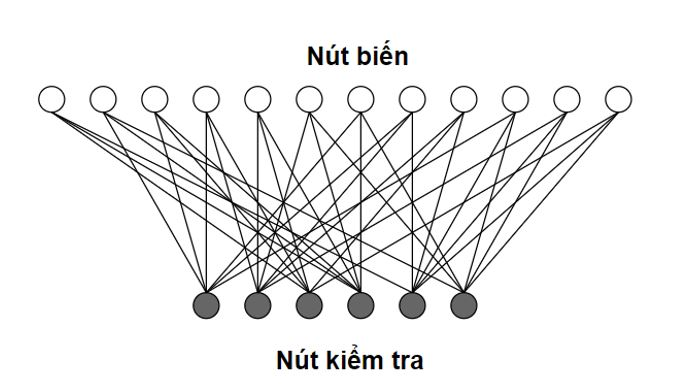
\includegraphics[width=10cm]{images/tanner2.JPG}
    \caption[Tanner graph cho ma trận kiểm tra chẵn lẻ ]{\bfseries\fontsize{12pt}{0pt} \selectfont Tanner graph cho ma trận kiểm tra chẵn lẻ} %[tên ở list figure]{tên chú thích ảnh}
    \label{hinh13}
\end{figure}  
    \item Sum-product là tên chung cho một lớp thuật toán giải mã Maximum Likelihood (ML). Thuật toán sử dụng thông tin kênh truyền và các giá trị từ kênh truyền. Thuật toán tạo ra một giá trị xác xuất cho mỗi bit nhận được và làm mới giá trị này sau nhiều lần lặp để tìm ước lượng cho bit đó.
    \item Sum-product xử lý lặp đi lặp lại các bit nhận được theo các bước nối liền nhau có thể nhìn thấy trên đồ hình Tanner để cải thiện độ tin cậy mỗi bit được giải mã.
    \item 	Để minh họa, hãy xét tin độ cậy một bit được giải mã được đo bằng xác xuất $P(x_N |Y),1\le n \le N$. Sau đó Log-Likelihood Ratio (LLR) của mỗi bit mã được tính bởi công thức:
    \begin{equation}\label{134}
        L(x_N)= log (\frac {P(x_N=0|Y)}{P(x_N=1|Y)})
    \end{equation}
    
    \item 	Trong mỗi lần lặp lại, một giá trị $r_{m \to n}$ được tính tại mỗi nút kiểm tra m theo chiều ngang và được chuyển cho tất cả các nút biến n nếu $n\in N\{m\}$. Tương tự, mỗi nút biến n sẽ gửi một giá trị $q_{n \to m}$ được tính theo chiều dọc đến tất cả các nút kiểm tra m nếu $n \in M\{n\}$.
    \item   Cần lưu ý rằng, việc tính toán sẽ được thực hiện tại các nút kiểm tra trước, rồi sau đó mới đến các bit node.
    \begin{figure}[H]
    \centering
    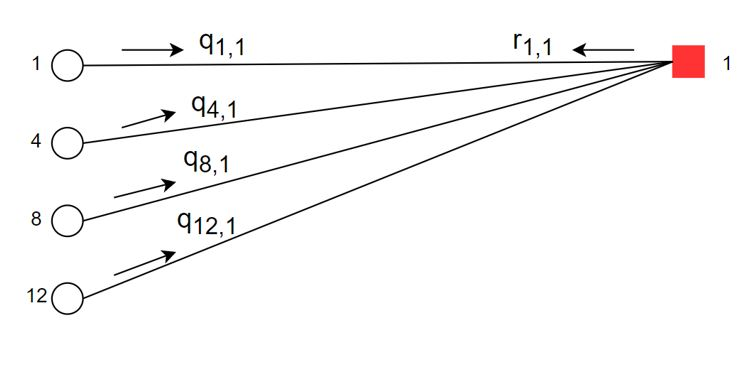
\includegraphics[width=10cm]{images/ktra3.JPG}
    \caption[Nút kiểm tra  1 nhận các giá trị $q_(n \to m)$ từ các bit node và tính toán trả lại giá trị $r_{(m \to n)}$ đến các bit node tương ứng ]{\bfseries\fontsize{12pt}{0pt} \selectfont Nút kiểm tra  1 nhận các giá trị $q_{(n \to m)}$ từ các bit node và tính toán trả lại giá trị $r_{(m \to n)}$ đến các bit node tương ứng} %[tên ở list figure]{tên chú thích ảnh}
    \label{hinh14}
\end{figure}
    \begin{figure}[H]
    \centering
    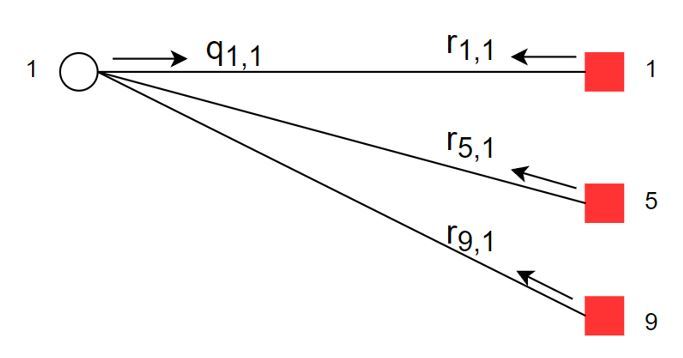
\includegraphics[width=10cm]{images/ktra4.JPG}
    \caption[Bit node 1 nhận các giá trị $r_{(m \to n)}$ từ các node kiểm tra, rồi tính toán và tính toán lại các giá trị $q_{(n \to m)}$ đến các node kiểm tra tương ứng ]{\bfseries\fontsize{12pt}{0pt} \selectfont Bit node 1 nhận các giá trị $r_{(m \to n)}$ từ các node kiểm tra, rồi tính toán và tính toán lại các giá trị $q_{(n \to m)}$ đến các node kiểm tra tương ứng} %[tên ở list figure]{tên chú thích ảnh}
    \label{hinh15}
\end{figure}
    \begin{figure}[H]
    \centering
    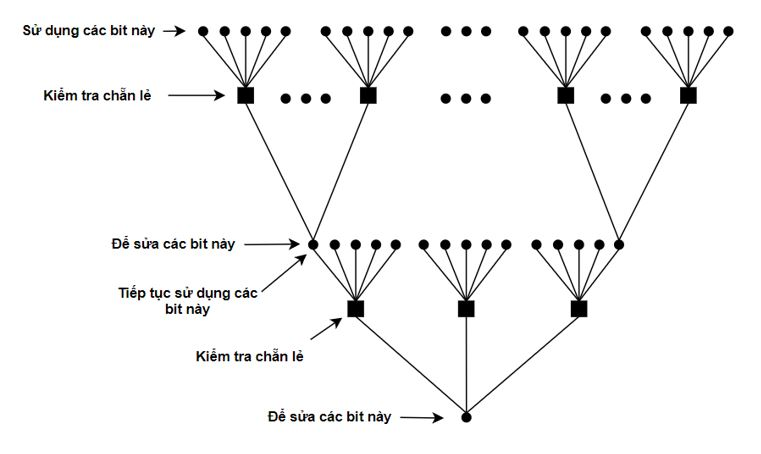
\includegraphics[width=10cm]{images/tongquan2.JPG}
    \caption[Tổng quan hơn về việc sửa lỗi bit dựa trên Tanner graph (Soft Decision Decoding) ]{\bfseries\fontsize{12pt}{0pt} \selectfont Tổng quan hơn về việc sửa lỗi bit dựa trên Tanner graph (Soft Decision Decoding)} %[tên ở list figure]{tên chú thích ảnh}
    \label{hinh16}
\end{figure}
    \item 	Từ mã ta sẽ ký hiệu là $X=[x_1,x_2,...,x_N]$, trong đó $x_N \in \{0,1\}$. Các giá trị LLR của vector nhận được tương ứng được biểu thị bằng $Y=[y_1,y_2,...,y_N ]$.
    \item 	Quá trình giải mã sử dụng thuật toán sum-product có thể được thực hiện theo các bước liên tiếp theo hình dưới đây.
    \begin{figure}[H]
    \centering
    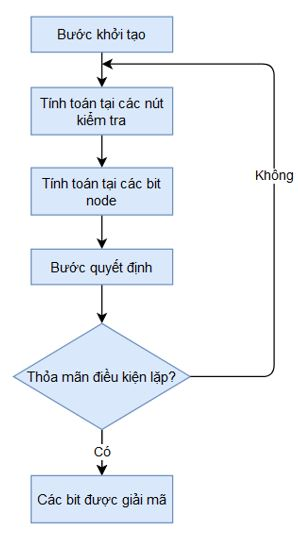
\includegraphics[width=8cm]{images/giaithuatSum.JPG}
    \caption[Giải thuật giải mã Sum-Product ]{\bfseries\fontsize{12pt}{0pt} \selectfont Giải thuật giải mã Sum-Product} %[tên ở list figure]{tên chú thích ảnh}
    \label{hinh17}
\end{figure}
    \begin{enumerate}
    \item 	Bước khởi tạo: Các giá trị ban đầu của LLR có thể nhận được từ đầu ra của bộ giải điều chế $y_n$. Các giá trị này được sử dụng làm $q_{n\to m}$  của lần lặp đầu tiên cho tới bước cập nhập nút kiểm tra.
    \item 	Tính toán tại các nút kiểm tra: Tại từng nút kiểm tra m, xử lý các giá trị đến từ các nút biến (bit node) $q_{n\to m}$ để tính toán các giá trị trả lời $r_{m\to n}$ cho mọi $n \in N\{m\}$. Vì vậy, đối với nút kiểm tra m:
       \begin{equation}\label{135}
           r_{(m \to n)} =  (\prod_{n \in N(m) \textbackslash n} sgn(q_{n \to m}) \times 2tanh^{-1}(\prod_{n \in N(m) \textbackslash n}tanh(\frac{|q_{n \to m|}}{2}))
       \end{equation}
    \item 	Tính toán tại các nút kiểm tra: Tại các nút biến n, xử lý các giá trị đến từ các nút kiểm tra  $r_{m\to n}$ để tính toán các giá trị trả lời $q_{n\to m}$  cho mọi $m \in N\{n\}$. Vì vậy, đối với nút biến n:
       \begin{equation}\label{136}
           q_{n \to m} = y_n+ \sum_{m \in M(n) \textbackslash m} r_{m \to n}(x_n)
       \end{equation}
    \item Bước quyết định: Đối với mỗi nút biến, các giá trị LLR được cập nhập theo công thức:
       \begin{equation}\label{137}
           L(x_n ) = y_n+ \sum_{m \in M(n)} r_{m \to n}(x_n)
       \end{equation}
      	Các giá trị LLR được áp dụng cho được áp dụng quyết định cứng để quyết định giá trị trả về. Ví dụ với kênh truyền BPSK thì 0 sẽ là ngưỡng để quyết định xem đó là -1 hay 1. Các giá trị LLR này sẽ được lặp đi lặp lại cho đến khi thỏa mãn điều kiện lặp. Điều kiện lặp có thể đạt được khi tiến hành kiểm tra Syndrome $Hx^T$ bằng 0 hoặc thỏa mãn điều kiện lặp tối đa. Như vậy quá trình lặp sẽ tiếp tục cho đến khi từ mã được giải thành công hoặc số lần lặp tối đa đã hết.

    \end{enumerate}
\end{itemize}
\cleardoublepage
\section*{CHƯƠNG 2. MÔ PHỎNG MATLAB}
\addcontentsline{toc}{section}{\numberline{}CHƯƠNG 2. MÔ PHỎNG MATLAB}
\setcounter{section}{2}
\setcounter{subsection}{0}
\setcounter{figure}{0}
\setcounter{table}{0}
\subsection{Thuật toán}
\subsubsection{Giải thuật Min-sum Product}
Để cải thiện tốc độ giải mã ta có thể chỉnh sửa lại thuật toán Sum-Product nhằm giảm độ phức tạp khi thực hiện của bộ giải mã.

Giải thuật Min-Sum Product sẽ có các bước và các phương trình giống như với giải thuật Sum-Product. Tuy nhiên, sẽ có sự thay đổi ở phương trình (1.24). Phương trình (1.24) sẽ được viết lại thành:
   \begin{equation}\label{138}
       r_{m \to n} = (\prod_{n \in N(m) \textbackslash n} sgn(q_{n \to m}) \times \min |q_{n \to m}|
   \end{equation}
\subsubsection{Kỹ thuật phân lớp}
Để cải thiện hiệu năng giải mã của thuật toán sum-product, ta sẽ áp dụng kỹ thuật phân lớp. Kỹ thuật này giúp bộ giải mã của ta đạt được thông lượng giải mã hiệu quả cao với độ phức tạp tính toán thấp.

Đối với mỗi lần lặp, chúng ta sẽ tính toán nút kiểm tra và nút biến trong một lớp. Việc giải mã sau đó diễn ra tuần tự. Điều này có nghĩa là ta sẽ tập hợp một số hàng của ma trận kiểm tra chẵn lẻ thành một lớp. Ma trận H sẽ được phân lớp như sau:
  \begin{equation}\label{139}
      H = 
      \begin{bmatrix}
        H_1 \\
        H_2 \\
        \vdots \\
        H_{N-K}
      \end{bmatrix}
  \end{equation}
 trong đó mỗi hàng trong ma trận H là một lớp.
 \begin{figure}[H]
    \centering
    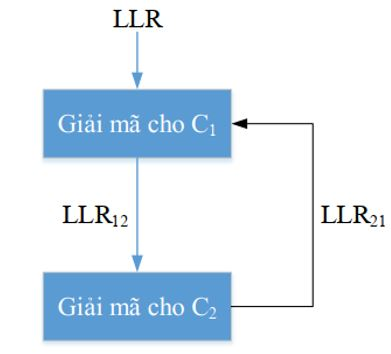
\includegraphics[width=10cm]{images/giaimaphanlop.JPG}
    \caption[Thuật toán giải mã với kỹ thuật phân lớp]{\bfseries\fontsize{12pt}{0pt} \selectfont Thuật toán giải mã với kỹ thuật phân lớp} %[tên ở list figure]{tên chú thích ảnh}
    \label{hinh21}
\end{figure}
 Hình trên minh họa sơ đồ giải mã của kỹ thuật phân lớp khi có 2 lớp: $C_1$ là từ mã được mã hóa từ $H_1$ và $C_2$ là từ mã được mã hóa từ $H_2$. Việc giải mã C1 sẽ sử dụng LLR trong vòng lặp đầu tiên, sau đó sẽ sử dụng $LLR_{21}$ sau khi đã cập nhập cột.
\subsection{Mô phỏng}
Mô phỏng cho hệ thống truyền thông được điều chế BPSK (Binary Phase Shift Keying) với nhiễu Gaussian trắng cộng (Additive White Gaussian Noise – AWGN) theo sơ đồ dưới đây
\begin{figure}[H]
    \centering
    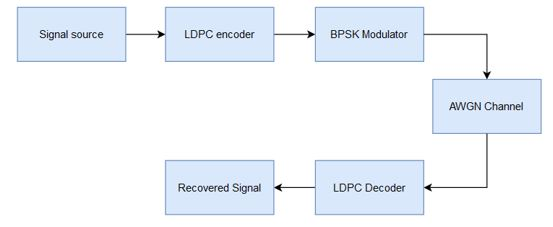
\includegraphics[width=12cm]{images/mohinh.JPG}
    \caption[Mô hình thực hiện việc điều chế, mã hóa, giải mã hóa với LDPC]{\bfseries\fontsize{12pt}{0pt} \selectfont Mô hình thực hiện việc điều chế, mã hóa, giải mã hóa với LDPC} %[tên ở list figure]{tên chú thích ảnh}
    \label{hinh22}
\end{figure}
   \begin{itemize}
       \item 	Ở đây ta sẽ thực hiện mô phỏng kênh truyền khi không thực hiện mã hóa LDPC và mã hóa LDPC với các lần lặp khác nhau.
       \item	Các hình 14, hình 15 và hình 16 là kết quả của việc thực hiện mã hóa LDPC với lần lặp là 8.
       \item 	Các hình 17 và hình 18 là kết quả so sánh giữa việc không thực hiện mã hóa LDPC và mã hóa LDPC với các lần lặp khác nhau.
       \item Việc mã hóa và giải mã hóa ở đây sẽ được thực hiện với ma trận BG1 với hệ số mở rộng Z là 16 và 100 khối bit truyền.
   \end{itemize}
   Code matlab được trình bày ở phần Phụ lục.
\subsection{Kết quả}
\begin{figure}[H]
    \centering
    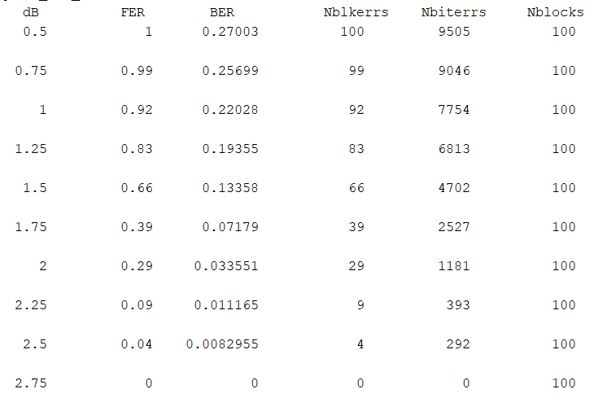
\includegraphics[width=12cm]{images/ketqua1.JPG}
    \caption[Kết quả mô phỏng với số lần lặp tối đa là 8]{\bfseries\fontsize{12pt}{0pt} \selectfont Kết quả mô phỏng với số lần lặp tối đa là 8} %[tên ở list figure]{tên chú thích ảnh}
    \label{hinh23}
\end{figure}
\begin{figure}[H]
    \centering
    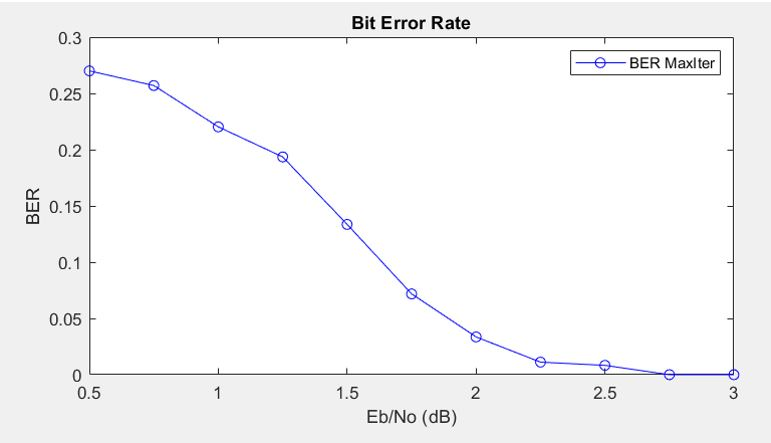
\includegraphics[width=12cm]{images/BER.JPG}
    \caption[BER theo Eb/N0¬ với số lần lặp tối đa là 8]{\bfseries\fontsize{12pt}{0pt} \selectfont BER theo Eb/N0¬ với số lần lặp tối đa là 8} %[tên ở list figure]{tên chú thích ảnh}
    \label{hinh24}
\end{figure}
\begin{figure}[H]
    \centering
    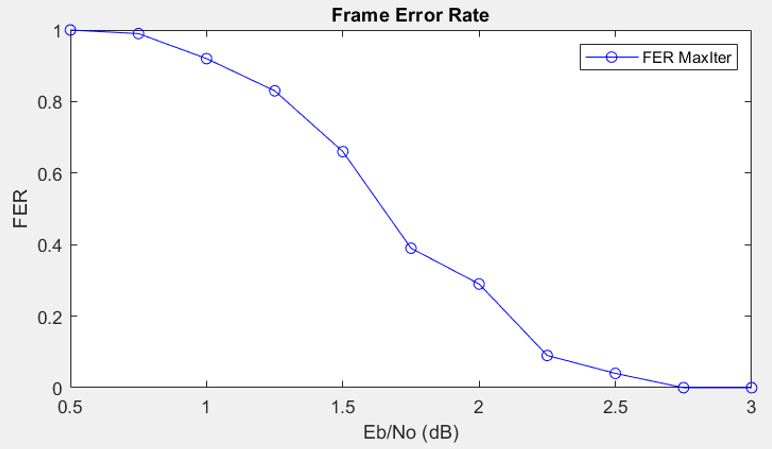
\includegraphics[width=12cm]{images/FER.JPG}
    \caption[FER theo Eb/N0¬ với số lần lặp tối đa là 8]{\bfseries\fontsize{12pt}{0pt} \selectfont FER theo Eb/N0¬ với số lần lặp tối đa là 8} %[tên ở list figure]{tên chú thích ảnh}
    \label{hinh25}
\end{figure}
\begin{figure}[H]
    \centering
    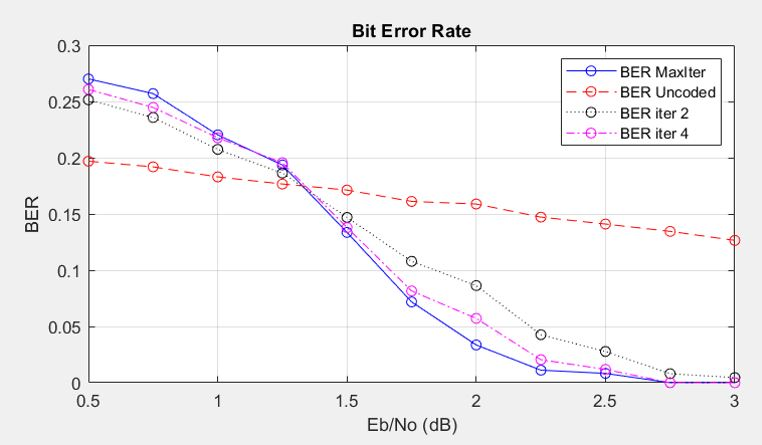
\includegraphics[width=12cm]{images/BER2.JPG}
    \caption[BER theo Eb/N0 với các trường hợp khác nhau]{\bfseries\fontsize{12pt}{0pt} \selectfont BER theo Eb/N0 với các trường hợp khác nhau} %[tên ở list figure]{tên chú thích ảnh}
    \label{hinh26}
\end{figure}
\begin{figure}[H]
    \centering
    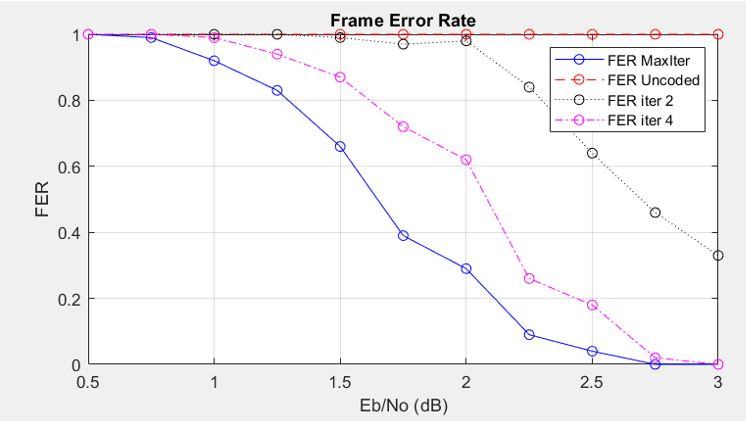
\includegraphics[width=12cm]{images/FER2.JPG}
    \caption[FER theo Eb/N0 với các trường hợp khác nhau]{\bfseries\fontsize{12pt}{0pt} \selectfont FER theo Eb/N0 với các trường hợp khác nhau} %[tên ở list figure]{tên chú thích ảnh}
    \label{hinh27}
\end{figure}
	Từ việc mô phỏng trên, ta có thể đưa ra một số nhận xét cụ thể như sau:
	\begin{itemize}
	    \item BER và FER sẽ giảm khi tỷ số Eb/N0 càng lớn
        \item Việc thực hiện mã hóa LDPC sẽ giúp cho tỷ lệ BER và FER giảm đi đáng kể so với việc không mã hóa.
        \item Số lần lặp càng lớn thì BER và FER càng giảm theo chiều tăng của Eb/N0.
	\end{itemize}
	
\cleardoublepage
\section*{THẢO LUẬN}
\phantomsection \addcontentsline{toc}{section}{\numberline {}THẢO LUẬN}
\thispagestyle{empty}
Nhóm em xin được trả lời một số câu hỏi của thầy đưa ra đối với đề tài này
  \begin{enumerate}
      \item Tại sao phải sử dụng ma trận thưa thớt?\\
      $\to$ Sử dụng ma trận thưa thớt sẽ giúp tăng tốc độ xử lý và tăng khả năng lưu trữ của bộ nhớ bởi ma trận thưa thớt sẽ chỉ lưu trữ tọa độ của các giá trị khác 0 và việc tính toán cũng sẽ chỉ dựa trên trên các giá trị khác 0 này.
      \item Mục đích của việc sử dụng ma trận cơ sở cùng với hệ số mở rộng?\\
      $\to$ Hệ số mở rộng giúp mở rộng ma trận cơ sở thành ma trận thưa thớt. Ma trận cơ sở khi mở rộng sẽ có không gian ma trận khá lớn, vì vậy để việc lưu trữ dễ hơn, người ta sử dụng ma trận cơ sở và hệ số mở rộng.
  \end{enumerate}

\cleardoublepage

\section*{PHỤ LỤC}
\phantomsection \addcontentsline{toc}{section}{\numberline {}PHỤ LỤC}
\texttt{\fontsize{11pt}{0pt}\selectfont Mã code mô phỏng}

\begin{tcolorbox}
\begin{minted}[
frame=lines,
framesep=2mm,
baselinestretch=1,
bgcolor=white,
fontsize=\footnotesize,
%linenos
]{matlab}
1.	Hàm dịch ma trận theo khối vào:
function y = mul_sh(x,k)
%x: Khoi vao
%k: -1 hoac so lan dich
%y: Khoi ra
if (k==-1)
    y = zeros(1,length(x));
else
    y = [x(k+1:end) x(1:k)];
end

\end{minted}
\end{tcolorbox}
\begin{tcolorbox}
\begin{minted}[
frame=lines,
framesep=2mm,
baselinestretch=1,
bgcolor=white,
fontsize=\footnotesize,
%linenos
]{matlab}
2.	Hàm Encoding cho từng vector message đầu vào:
function cword = ldpc_encode(B,z,msg)
%B: Ma tran co so
%z: He so mo rong
%msg: message vector, length = (#cols(B)-#rows(B))*z
%cword: codeword vector, length = #cols(B)*z
 
[m,n] = size(B);
 
cword = zeros(1,n*z);
cword(1:(n-m)*z) = msg;
 
%Ma hoa duong cheo kep
temp = zeros(1,z);
for i = 1:4 %row 1 to 4
    for j = 1:n-m %message columns
        temp = mod(temp + mul_sh(msg((j-1)*z+1:j*z),B(i,j)),2);
    end
end
if B(2,n-m+1) == -1
    p1_sh = B(3,n-m+1);
else
    p1_sh = B(2,n-m+1);
end
cword((n-m)*z+1:(n-m+1)*z) = mul_sh(temp,z-p1_sh); %p1
%Tim p2, p3, p4
for i = 1:3
    temp = zeros(1,z);
    for j = 1:n-m+i
        temp = mod(temp + mul_sh(cword((j-1)*z+1:j*z),B(i,j)),2);
    end
    cword((n-m+i)*z+1:(n-m+i+1)*z) = temp;
end
%Cac bit chan le con lai
for i = 5:m
    temp = zeros(1,z);
    for j = 1:n-m+4
        temp = mod(temp + mul_sh(cword((j-1)*z+1:j*z),B(i,j)),2);        
    end
    cword((n-m+i-1)*z+1:(n-m+i)*z) = temp;    
end

\end{minted}
\end{tcolorbox}
    
\begin{tcolorbox}
\begin{minted}[
frame=lines,
framesep=2mm,
baselinestretch=1,
bgcolor=white,
fontsize=\footnotesize,
%linenos
]{matlab}

3.	Decoding:
clear
close all
format short g
 
MaxItrs = 8;
 
%Basegraphnumber_j_z
load base_matrices/NR_1_0_16.txt
B = NR_1_0_16;
[mb,nb] = size(B);
z = 16;
 
Slen = sum(B(:)~=-1); %So luong cac gia tri khac -1 trong B
min_reg = zeros(max(sum(B ~= -1,2)),z); %Thanh ghi luu cac gia tri minsum
k = (nb-mb)*z; %So cot bit message trong B
n = nb*z; %So cot bit codeword trong B
Rate = k/n;  %Toc do
 
 
dB=[0.5:0.25:3];              % Khoang SNR chay theo dB
FER=zeros(1,length(dB));      % Mang luu tru Frame Error Rate
BER=zeros(1,length(dB));      % Mang luu tru Bit Error Rate
 
FER_uncoded=zeros(1,length(dB));% Mang luu tru Frame Error Rate khong ma hoa
BER_uncoded=zeros(1,length(dB));% Mang luu tru Bit Error Rate khong ma hoa
 
FER_iter_2=zeros(1,length(dB));% Mang luu tru Frame Error Rate voi lan lap 2
BER_iter_2=zeros(1,length(dB));% Mang luu tru Bit Error Rate voi lan lap 2
 
FER_iter_4=zeros(1,length(dB));% Mang luu tru Frame Error Rate voi lan lap 4
BER_iter_4=zeros(1,length(dB));% Mang luu tru Bit Error Rate voi lan lap 4
 
EbNo=10.^(dB/10);   % Eb/No doi tu dB thanh thap phan
 
 
 
Nblocks = 100;   % So luong Block Message mo phong
disp('  dB   FER   BER    Nblkerrs   Nbiterrs    Nblocks')
for g=1:length(EbNo) % Vong lap de test trong khoang SNR
Nbiterrs = 0; Nblkerrs = 0; 
    Nbiterrs_uncoded = 0; Nblkerrs_uncoded = 0; 
    Nbiterrs_iter_2 = 0; Nblkerrs_iter_2 = 0; 
    Nbiterrs_iter_4 = 0; Nblkerrs_iter_4 = 0; 
    sigma = sqrt(1/(2*Rate*EbNo(g)));
    for i = 1: Nblocks
        msg = randi([0 1],1,k); %Tao k-bit message ngau nhien
        %msg = zeros(1,k); %all-zero message
        %cword = zeros(1,n); %all-zero codeword
        
        %Encoding 
        cword = ldpc_encode(B,z,msg);
        cword = cword(1:n);  
        s = 1 - 2 * cword; %Ma hoa BPSK
        r = s + sigma * randn(1,n); %AWGN channel I
\end{minted}
\end{tcolorbox}

\begin{tcolorbox}
\begin{minted}[
frame=lines,
framesep=2mm,
baselinestretch=1,
bgcolor=white,
fontsize=\footnotesize,
%linenos
]{matlab}
%Soft-decision, Layer decoding
        L = r; %Tong cac belief
        itr = 0; %so lan lap hien tai
        R = zeros(Slen,z); %Thanh ghi chua du lieu xu ly tren hang
        
        % Thuc hien Layer Decoding
        while itr < MaxItrs
            Ri = 0;
            for lyr = 1:mb %lyr la layer, mac dinh la 1
                ti = 0; %so luong cac gia tri khac -1 tai row=lyr
                for col = find(B(lyr,:) ~= -1)
                       ti = ti + 1;
                       Ri = Ri + 1;
                       %Subtraction (Thuc hien phep tru)
                       L((col-1)*z+1:col*z) = L((col-1)*z+1:col*z)-R(Ri,:);
                       %can chinh lai gia tri hang va luu tru trong min_reg
                     min_reg(ti,:) = mul_sh(L((col-1)*z+1:col*z),B(lyr,col)); 
                end
                %minsum tai min_reg: ti x z
                for i1 = 1:z %min_reg(1:ti,i1)
                    [min1,pos] = min(abs(min_reg(1:ti,i1))); 
                    %Cuc tieu thu nhat theo gia tri tuyet doi
                    min2 = min(abs(min_reg([1:pos-1 pos+1:ti],i1))); 
                    %Cuc tieu thu 2 theo gia tri tuyet doi
                    S = sign(min_reg(1:ti,i1)); %Luu tru dau cua 1 hang
                    parity = prod(S); %Tich cac dau cua 1 hang
                    min_reg(1:ti,i1) = min1; 
                    %Thay the thanh gia tri tuyet doi min1
                    min_reg(pos,i1) = min2;
                %Thay the cho vi tri cua min1 thanh gia tri tuyet doi min2
                    min_reg(1:ti,i1) = parity*S.*min_reg(1:ti,i1); 
                    %Nhan them dau cua hang
                end
                %Thuc hien hinh lai gia tri cot, addition va luu tru trong R
                Ri = Ri - ti; %reset Ri
                ti = 0;
                for col = find(B(lyr,:) ~= -1)
                        Ri = Ri + 1;
                        ti = ti + 1;
                        %Can chinh gia tri cot
                        R(Ri,:) = mul_sh(min_reg(ti,:),z-B(lyr,col));
                        %Addition (Thuc hien phep cong)
                        L((col-1)*z+1:col*z) = L((col-1)*z+1:col*z)+R(Ri,:);
                end
            end      
            if itr == 2
               msg_iter_2 = L(1:k)<0;
            end
            if itr == 4
               msg_iter_4 = L(1:k)<0;
            end      
\end{minted}
\end{tcolorbox}

\begin{tcolorbox}
\begin{minted}[
frame=lines,
framesep=2mm,
baselinestretch=1,
bgcolor=white,
fontsize=\footnotesize,
%linenos
]{matlab}

            itr = itr + 1;       
        end
        msg_cap = L(1:k) < 0; %Quyet dinh
        uncoded_msg = r(1:k) < 0;
        %Dem loi
        Nerrs_uncoded = sum(msg ~= uncoded_msg);
        Nerrs_iter_2 = sum(msg ~= msg_iter_2);
        Nerrs_iter_4 = sum(msg ~= msg_iter_4);
        Nerrs = sum(msg ~= msg_cap);
        if Nerrs > 0
            Nbiterrs = Nbiterrs + Nerrs;
            Nblkerrs = Nblkerrs + 1;
        end
        if Nerrs_uncoded > 0
            Nbiterrs_uncoded = Nbiterrs_uncoded + Nerrs_uncoded;
            Nblkerrs_uncoded = Nblkerrs_uncoded + 1;
        end
        if Nerrs_iter_2 > 0
            Nbiterrs_iter_2 = Nbiterrs_iter_2 + Nerrs_iter_2;
            Nblkerrs_iter_2 = Nblkerrs_iter_2 + 1;
        end
        if Nerrs_iter_4 > 0
            Nbiterrs_iter_4 = Nbiterrs_iter_4 + Nerrs_iter_4;
            Nblkerrs_iter_4 = Nblkerrs_iter_4 + 1;
        end  
    end
   
    BER(g) = Nbiterrs/k/Nblocks;
    FER(g) = Nblkerrs/Nblocks;
    
    BER_uncoded(g) = Nbiterrs_uncoded/k/Nblocks;
    FER_uncoded(g) = Nblkerrs_uncoded/Nblocks;
    
    BER_iter_2(g) = Nbiterrs_iter_2/k/Nblocks;
    FER_iter_2(g) = Nblkerrs_iter_2/Nblocks;
    
    BER_iter_4(g) = Nbiterrs_iter_4/k/Nblocks;
    FER_iter_4(g) = Nblkerrs_iter_4/Nblocks;
 
    %disp([EbNodB FER_sim BER_sim Nblkerrs Nbiterrs Nblocks])
    disp([dB(g) FER(g) BER(g) Nblkerrs Nbiterrs Nblocks])
end
    
subplot(2,2,1)
plot(dB,BER,'b-o')
legend('BER MaxIter ');
title('Bit Error Rate')
ylabel('BER')
xlabel('Eb/No (dB)')

\end{minted}
\end{tcolorbox}

\begin{tcolorbox}
\begin{minted}[
frame=lines,
framesep=2mm,
baselinestretch=1,
bgcolor=white,
fontsize=\footnotesize,
%linenos
]{matlab}

subplot(2,2,2)
plot(dB,BER,'b-o')
hold on;
plot(dB,BER_uncoded,'r--o')
plot(dB,BER_iter_2,'k:o')
plot(dB,BER_iter_4,'m-.o')
legend('BER MaxIter ','BER Uncoded','BER iter 2','BER iter 4');
title('Bit Error Rate')
ylabel('BER')
xlabel('Eb/No (dB)')
grid
%figure
hold off;
 
subplot(2,2,3)
plot(dB,FER,'b-o')
legend('FER MaxIter ');
title('Frame Error Rate')
ylabel('FER')
xlabel('Eb/No (dB)')
 
subplot(2,2,4)
plot(dB,FER,'b-o')
hold on;
plot(dB,FER_uncoded,'r--o')
plot(dB,FER_iter_2,'k:o')
plot(dB,FER_iter_4,'m-.o')
legend('FER MaxIter ','FER Uncoded','FER iter 2','FER iter 4');
title('Frame Error Rate')
ylabel('FER')
xlabel('Eb/No (dB)')
grid
\end{minted}
\end{tcolorbox}

\end{document}

